\section{Experiments}

% As with other methods, we observe that introducing a silhouette term into the network loss before the model's pose has been somewhat solved can result in unsatisfactory local minima. We overcome this by using a pre-training stage with the following loss terms:


In this section, the WLDO method is compared against competitive baselines. The protocol for evaluation is described first, followed by a quantitative and qualitative evaluation.

\subsection{Evaluation protocol}

Evaluation is based on the StanfordExtra dataset introduced earlier in the chapter, which contains 8,476 images for 120 breeds. These images are divided per-breed into an 80\%/20\% train and test split.

Two primary evaluation metrics are considered. IoU is the intersection-over-union of the projected model silhouette compared to the ground truth annotation and indicates the quality of the reconstructed 3D shape. Percentage of Correct Keypoints (PCK) computes the percentage of joints which are within a normalized distance (based on square root of 2D silhouette area) to the ground truth locations, and evaluates the quality of reconstructed 3D pose. In addition, PCK results are produced for various joint groups (legs, tail, ears, face) in order to compare the reconstruction accuracy for different parts of the dog. Also used for evaluation is a new comparison metric \emph{PCK-MAX}. This protocol is similar to the Percentage of Correct Keypoints (PCK) metric~\cite{yang2013articulated} but incorporates the `invisible' ground-truth points. The standard PCK metric ignores these points, meaning even correct 3D reconstructions will receive no credit. PCK-MAX instead assumes reconstructed 3D points for missing ground-truth data are correct, providing an interesting upper bound.

\subsection{Training procedure}

The WLDO network is trained in two stages. The first omits the silhouette loss which tends to lead the network to unsatisfactory local minima if applied too early. With the silhouette loss turned off, it is satisfactory to use the simple unimodal prior (and without EM) for this preliminary stage since there is no loss to specifically encourage a strong shape alignment. After this, the silhouette loss and mixture prior with $M=10$ clusters are introduced, and expectation maximization updates are applied every 50 epochs. The first stage is trained for 250 epochs and the second stage for 150. The entire training procedure takes approximately 96 hours on a single P100 GPU.

Recall that the training objective for our end-to-end system for predicting SMBLD parameters consistent with a monocular dog input image is given by:

\begin{equation}
    \L{opt}=\L{joints}+\L{sil}+\L{pose}+\L{shape}+\L{mixture}
\end{equation}

Each loss term is weighted with a scalar $\W{}$. The following details the specific weights used for each training stage:

\ss{Stage 1.} $\W{joints}=10.0,\W{pose}=1.0,\W{shape}=1.0,\W{sil}=0.0,\W{mixture}=0.0$. This stage is trained for 250 epochs using the Adam optimizer, with learning rate set to $10^{-4}$. 
\ss{Stage 2.} $\W{joints}=10.0,\W{pose}=0.5,\W{shape}=0.0,\W{sil}=100.0,\W{mixture}=0.1$. This stage is trained for 150 epochs and run the described EM update step every $K=50$ epochs. The number of clusters $M=10$ was selected based on a grid search over $M=1,5,10,25$ with IoU scores compared. The Adam optimizer is again applied with learning rate to $10^{-5}$.

To begin, WLDO is compared with various baseline methods. 3D Menagerie (3D-M)~\cite{zuffi2017menagerie} is an approach which fits the 3D SMAL model using per-image energy minimization. Creatures Great and SMAL (CGAS)~\cite{biggs2018creatures} is a three-stage method, which employs a joint predictor on silhouette renderings from synthetic 3D dogs, applies a genetic algorithm to clean predictions, and finally applies the SMAL optimizer to produce the 3D mesh.

At test-time both 3D-M and CGAS rely on manually-provided segementation masks, and 3D-M also relies on hand-clicked keypoints. In order to produce a fair comparison, we produce a set of \emph{predicted} keypoints for StanfordExtra by training the Stacked Hourglass Network~\cite{newell2016stacked} with 8 stacks and 1 block, and \emph{predicted} segmentation masks using DeepLab v3+~\cite{deeplabv3plus}. The Stacked Hourglass Network achieves 71.4\% PCK score, DeepLab v3+ achieves 83.4\% IoU score and the CGAS joint predictor achieves 41.8\% PCK score. 

%All methods are trained from scratch and evaluated on our Stanford Dog validation set.

% \begin{table}[]
\centering
\begin{tabular}{@{}lcc@{}}
\toprule
\multicolumn{1}{l}{Method} & 
\multicolumn{1}{c}{IoU} & 
\multicolumn{1}{c}{PCK} 
\\ 
\midrule
DeepLab v3+ & 83.4 & --- \\
HourglassNet & --- & 71.4 \\
CGAS Joint Predictor & --- & 51.8 \\
\bottomrule 
\end{tabular}
\vspace{1em}
\caption{\label{tab:othernetworks}\textbf{Competitive Networks}. We evaluate the performance of Stacked Hourglass Network with 8 stacks and 1 block and DeepLab v3+ trained on our Stanford Dog training set and evaluated on the test set. We train CGAS on the synthetic data and evaluate on ground truth segmentations in the Stanford Dog test set.}
\end{table}
% \begin{table}[]
\centering
\begin{tabular}{@{}lcc@{}}
\toprule
\multicolumn{1}{l}{Method} & 
\multicolumn{1}{c}{IoU} & 
\multicolumn{1}{c}{PCK} 
\\ 
\midrule
DeepLab v3+ & 83.4 & --- \\
HourglassNet & --- & 71.4 \\
CGAS Joint Predictor & --- & 51.8 \\
\bottomrule 
\end{tabular}
\vspace{1em}
\caption{\label{tab:othernetworks}\textbf{Competitive Networks}. We evaluate the performance of Stacked Hourglass Network with 8 stacks and 1 block and DeepLab v3+ trained on our Stanford Dog training set and evaluated on the test set. We train CGAS on the synthetic data and evaluate on ground truth segmentations in the Stanford Dog test set.}
\end{table}

Table~\ref{tab:baselinesfix}, \Cref{fig:comparison_1} and \Cref{fig:comparison_2} show the comparison against competitive methods. For full examination, results for 3D-M and CGAS are additionally provided in the scenario that ground-truth keypoints and/or segmentations are available at test time. 

The results show our end-to-end method outperforms the competitors when they are provided with predicted keypoints/segmentations (white rows). The WLDO method therefore achieves a new state-of-the-art on this 3D reconstruction task. In addition, the method is shown to achieve improved average IoU/PCK scores than competitive methods, even when competitors are provided ground truth annotations at test time (grey rows). Also demonstrated is the wider applicability of two contributions of this chapter (scale parameters and improved prior) in the improved performance of the 3D-M method when these are incorporated. Finally, WLDO's test-time speed is significantly faster than competitive methods as no subsequent energy minimization procedure is required. 

\begin{table}[]
{
    \small
    \centering
    \begin{tabular}{@{}lcccccccc@{}}
    \toprule
    \multicolumn{1}{l}{Method} & 
    \multicolumn{1}{c}{Kps} & 
    \multicolumn{1}{c}{Seg} & 
    \multicolumn{1}{c}{IoU} & 
    \multicolumn{5}{c}{PCK @ 0.15} \\
    \multicolumn{4}{c}{} &
    \multicolumn{1}{c}{Avg} &
    \multicolumn{1}{c}{Legs} &
    \multicolumn{1}{c}{Tail} &
    \multicolumn{1}{c}{Ears} &
    \multicolumn{1}{c}{Face} \\
    \midrule
    \rowcolor{comp} 3D-M~\cite{zuffi2017menagerie} & Pred & Pred & 69.9 & 69.7 & 68.3 & 68.0 & 57.8 & 93.7 \\
    \rowcolor{notcomp} 3D-M & GT & GT & 71.0 & 75.6 & 74.2 & 89.5 & 60.7 & 98.6 \\
    \rowcolor{notcomp} 3D-M & GT & Pred & 70.7 & 75.5 & 74.1 & 88.1 & 60.2 & 98.7 \\
    \rowcolor{notcomp} 3D-M & Pred & GT & 70.5 & 70.3 & 69.0 & 69.4 & 58.5 & 94.0 \\
    \hline
    \rowcolor{comp} CGAS~\cite{biggs2018creatures} & CGAS & Pred & 63.5 & 28.6 & 30.7 & 34.5 & 25.9 & 24.1 \\
    \rowcolor{notcomp} CGAS & CGAS & GT & 64.2 & 28.2 & 30.1 & 33.4 & 26.3 & 24.5 \\
    \hline
    \rowcolor{comp} 3D-M + scaling & Pred & Pred & 70.4 & 70.9 & 69.8 & 66.9 & 59.7 & 94.0 \\
    \rowcolor{comp} 3D-M + scaling + EM prior & Pred & Pred & 71.8 & 73.4 & 72.5 & \textbf{70.3} & 62.6 & \textbf{94.1} \\
    \hline
    \rowcolor{comp} \textbf{Ours} & --- & --- & \textbf{74.2} & \textbf{78.8} & \textbf{76.4} & 63.9 & \textbf{78.1} & 92.1 \\
    \bottomrule 
    \end{tabular}
    \vspace{1em}
    \caption[]{\label{tab:baselinesfix}\textbf{Baseline comparisons.} PCK and silhouette IOU scores are shown for SOTA methods under varying conditions. Directly comparable baseline methods (requiring only an input image) are highlighted. \emph{Pred} keypoints generated with Hourglass-Net~\cite{newell2016stacked} and segmentations with DeepLab v3+~\cite{journals/corr/ChenPK0Y16}. 3D-M/CGAS are also analysed when they have access to ground-truth keypoints and/or segmentation masks. We also analyse adding this paper's innovations (scale parameters and EM prior) to 3D-M~\cite{zuffi2017menagerie}.}
}
\end{table}


\newcolumntype{?}{!{\vrule width 1pt}}

% \newcommand\sfac{0.082}
% \newcommand\spacercomp{4mm}
\begin{figure*}[ht!]
    \centering
    \setkeys{Gin}{width=\linewidth}
    \renewcommand\tabularxcolumn[1]{>{\Centering}m{\sfac\linewidth}} % set all columns to be centered v & hwise, with a fixed length
    \newcolumntype{D}{ >{\centering\arraybackslash} m{\imgwidthcomp} }
    \newcolumntype{E}{ >{\centering\arraybackslash} m{\labelwidthcomp} }

    % \begin{tabularx}{\textwidth}{c*{5}{X}@{\hspace{\spacercomp}}*{5}{X}c}
    % \begin{tabularx}{\textwidth}{c*{5}{X}}
    \begin{tabularx}{\textwidth}{EDDDDD}
      \textbf{Ours} &
      \includegraphics{ours_sup/n02086646-Blenheim_spaniel/orig/n02086646_1476.jpg} &
      \includegraphics{ours_sup/n02086646-Blenheim_spaniel/fit/n02086646_1476.jpg} &
      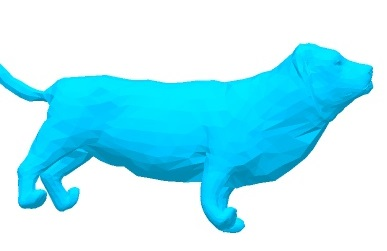
\includegraphics{ours_sup/n02086646-Blenheim_spaniel/model/n02086646_1476_crop.jpg} &
      \includegraphics{ours_sup/n02086646-Blenheim_spaniel/joints/n02086646_1476.jpg} &
      \includegraphics{ours_sup/n02086646-Blenheim_spaniel/segs/n02086646_1476.jpg} \\
      

      3D-M &
      \includegraphics{comp_sup/smal/n02086646-Blenheim_spaniel/orig/n02086646_1476.jpg} &
      \includegraphics{comp_sup/smal/n02086646-Blenheim_spaniel/fit/n02086646_1476.jpg} &
      \includegraphics{comp_sup/smal/n02086646-Blenheim_spaniel/model/n02086646_1476_fixed_crop.jpg} &
      \includegraphics{comp_sup/smal/n02086646-Blenheim_spaniel/joints/n02086646_1476.jpg} &
      \includegraphics{comp_sup/smal/n02086646-Blenheim_spaniel/segs/n02086646_1476.jpg} \\
      

      CGAS &
      \includegraphics{comp_sup/cgas/n02086646-Blenheim_spaniel/orig/n02086646_1476.jpg} &
      \includegraphics{comp_sup/cgas/n02086646-Blenheim_spaniel/fit/n02086646_1476.jpg} &
      \includegraphics{comp_sup/cgas/n02086646-Blenheim_spaniel/model/n02086646_1476_fixed_crop.jpg} &
      \includegraphics{comp_sup/cgas/n02086646-Blenheim_spaniel/joints/n02086646_1476.jpg} &
      \includegraphics{comp_sup/cgas/n02086646-Blenheim_spaniel/segs/n02086646_1476.jpg} \\
      %\hspace{\spacercomp}
     
      \textbf{Ours} &
      \includegraphics{ours_sup/n02087394-Rhodesian_ridgeback/orig/n02087394_831.jpg} &
      \includegraphics{ours_sup/n02087394-Rhodesian_ridgeback/fit/n02087394_831.jpg} &
      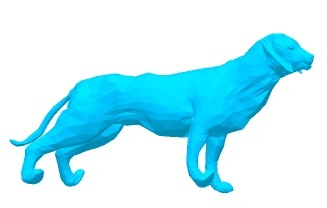
\includegraphics{ours_sup/n02087394-Rhodesian_ridgeback/model/n02087394_831_crop.jpg} &
      \includegraphics{ours_sup/n02087394-Rhodesian_ridgeback/joints/n02087394_831.jpg} &
      \includegraphics{ours_sup/n02087394-Rhodesian_ridgeback/segs/n02087394_831.jpg} \\

      3D-M &
      %\hspace{\spacercomp}
      \includegraphics{comp_sup/smal/n02087394-Rhodesian_ridgeback/orig/n02087394_831.jpg} &
      \includegraphics{comp_sup/smal/n02087394-Rhodesian_ridgeback/fit/n02087394_831.jpg} &
      \includegraphics{comp_sup/smal/n02087394-Rhodesian_ridgeback/model/n02087394_831_fixed_crop.jpg} &
      \includegraphics{comp_sup/smal/n02087394-Rhodesian_ridgeback/joints/n02087394_831.jpg} &
      \includegraphics{comp_sup/smal/n02087394-Rhodesian_ridgeback/segs/n02087394_831.jpg} \\

      CGAS &
      \includegraphics{comp_sup/cgas/n02087394-Rhodesian_ridgeback/orig/n02087394_831.jpg} &
      \includegraphics{comp_sup/cgas/n02087394-Rhodesian_ridgeback/fit/n02087394_831.jpg} &
      \includegraphics{comp_sup/cgas/n02087394-Rhodesian_ridgeback/model/n02087394_831_fixed_crop.jpg} &
      \includegraphics{comp_sup/cgas/n02087394-Rhodesian_ridgeback/joints/n02087394_831.jpg} &
      \includegraphics{comp_sup/cgas/n02087394-Rhodesian_ridgeback/segs/n02087394_831.jpg} \\
      
      % & 
      & (a) & (b) & (c) & (d) & (e) \\
      %\hspace{\spacercomp} 
      % (a) & (b) & (c) & (d) & (e) \\
    \end{tabularx}
    %
    \caption{%
    \textbf{Qualitiative comparison to SOTA.} 
    Row 1: \textbf{Ours}, 
    Row 2: 3D-M~\cite{zuffi2017menagerie}, 
    Row 3: CGAS~\cite{biggs2018creatures}. 
    (a) input image, (b) predicted 3D mesh, (c) canonical view 3D mesh, 
    (d) reprojected model joints and (e) silhouette reprojection error. 
    }
    \label{fig:comparison_1}
\end{figure*}

\newcolumntype{?}{!{\vrule width 1pt}}

% \newcommand\sfac{0.082}
% \newcommand\spacercomp{4mm}
\begin{figure*}[ht!]
    \centering
    \setkeys{Gin}{width=\linewidth}
    \renewcommand\tabularxcolumn[1]{>{\Centering}m{\sfac\linewidth}} % set all columns to be centered v & hwise, with a fixed length
    \newcolumntype{D}{ >{\centering\arraybackslash} m{\imgwidthcomp} }
    \newcolumntype{E}{ >{\centering\arraybackslash} m{\labelwidthcomp} }

    % \begin{tabularx}{\textwidth}{c*{5}{X}@{\hspace{\spacercomp}}*{5}{X}c}
    % \begin{tabularx}{\textwidth}{c*{5}{X}}
    \begin{tabularx}{\textwidth}{EDDDDD}
      % \textbf{Ours} &
      % \includegraphics{ours_sup/n02086646-Blenheim_spaniel/orig/n02086646_1476.jpg} &
      % \includegraphics{ours_sup/n02086646-Blenheim_spaniel/fit/n02086646_1476.jpg} &
      % 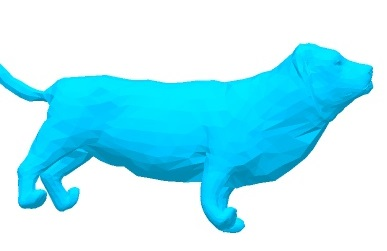
\includegraphics{ours_sup/n02086646-Blenheim_spaniel/model/n02086646_1476_crop.jpg} &
      % \includegraphics{ours_sup/n02086646-Blenheim_spaniel/joints/n02086646_1476.jpg} &
      % \includegraphics{ours_sup/n02086646-Blenheim_spaniel/segs/n02086646_1476.jpg} \\
      

      % 3D-M &
      % \includegraphics{comp_sup/smal/n02086646-Blenheim_spaniel/orig/n02086646_1476.jpg} &
      % \includegraphics{comp_sup/smal/n02086646-Blenheim_spaniel/fit/n02086646_1476.jpg} &
      % \includegraphics{comp_sup/smal/n02086646-Blenheim_spaniel/model/n02086646_1476_fixed_crop.jpg} &
      % \includegraphics{comp_sup/smal/n02086646-Blenheim_spaniel/joints/n02086646_1476.jpg} &
      % \includegraphics{comp_sup/smal/n02086646-Blenheim_spaniel/segs/n02086646_1476.jpg} \\
      

      % CGAS &
      % \includegraphics{comp_sup/cgas/n02086646-Blenheim_spaniel/orig/n02086646_1476.jpg} &
      % \includegraphics{comp_sup/cgas/n02086646-Blenheim_spaniel/fit/n02086646_1476.jpg} &
      % \includegraphics{comp_sup/cgas/n02086646-Blenheim_spaniel/model/n02086646_1476_fixed_crop.jpg} &
      % \includegraphics{comp_sup/cgas/n02086646-Blenheim_spaniel/joints/n02086646_1476.jpg} &
      % \includegraphics{comp_sup/cgas/n02086646-Blenheim_spaniel/segs/n02086646_1476.jpg} \\
      % %\hspace{\spacercomp}
     
      % \textbf{Ours} &
      % \includegraphics{ours_sup/n02087394-Rhodesian_ridgeback/orig/n02087394_831.jpg} &
      % \includegraphics{ours_sup/n02087394-Rhodesian_ridgeback/fit/n02087394_831.jpg} &
      % 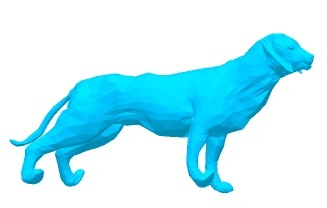
\includegraphics{ours_sup/n02087394-Rhodesian_ridgeback/model/n02087394_831_crop.jpg} &
      % \includegraphics{ours_sup/n02087394-Rhodesian_ridgeback/joints/n02087394_831.jpg} &
      % \includegraphics{ours_sup/n02087394-Rhodesian_ridgeback/segs/n02087394_831.jpg} \\

      % 3D-M &
      % %\hspace{\spacercomp}
      % \includegraphics{comp_sup/smal/n02087394-Rhodesian_ridgeback/orig/n02087394_831.jpg} &
      % \includegraphics{comp_sup/smal/n02087394-Rhodesian_ridgeback/fit/n02087394_831.jpg} &
      % \includegraphics{comp_sup/smal/n02087394-Rhodesian_ridgeback/model/n02087394_831_fixed_crop.jpg} &
      % \includegraphics{comp_sup/smal/n02087394-Rhodesian_ridgeback/joints/n02087394_831.jpg} &
      % \includegraphics{comp_sup/smal/n02087394-Rhodesian_ridgeback/segs/n02087394_831.jpg} \\

      % CGAS &
      % \includegraphics{comp_sup/cgas/n02087394-Rhodesian_ridgeback/orig/n02087394_831.jpg} &
      % \includegraphics{comp_sup/cgas/n02087394-Rhodesian_ridgeback/fit/n02087394_831.jpg} &
      % \includegraphics{comp_sup/cgas/n02087394-Rhodesian_ridgeback/model/n02087394_831_fixed_crop.jpg} &
      % \includegraphics{comp_sup/cgas/n02087394-Rhodesian_ridgeback/joints/n02087394_831.jpg} &
      % \includegraphics{comp_sup/cgas/n02087394-Rhodesian_ridgeback/segs/n02087394_831.jpg} \\
      
      \textbf{Ours} &
      \includegraphics{ours_sup/n02091134-whippet/orig/n02091134_16201.jpg} &
      \includegraphics{ours_sup/n02091134-whippet/fit/n02091134_16201.jpg} &
      \includegraphics{ours_sup/n02091134-whippet/model/n02091134_16201_crop.jpg} &
      \includegraphics{ours_sup/n02091134-whippet/joints/n02091134_16201.jpg} &
      \includegraphics{ours_sup/n02091134-whippet/segs/n02091134_16201.jpg} \\


      3D-M & 
      \includegraphics{comp_sup/smal/n02091134-whippet/orig/n02091134_16201.jpg} &
      \includegraphics{comp_sup/smal/n02091134-whippet/fit/n02091134_16201.jpg} &
      \includegraphics{comp_sup/smal/n02091134-whippet/model/n02091134_16201_fixed_crop.jpg} &
      \includegraphics{comp_sup/smal/n02091134-whippet/joints/n02091134_16201.jpg} &
      \includegraphics{comp_sup/smal/n02091134-whippet/segs/n02091134_16201.jpg} \\
      
      
      CGAS &
      \includegraphics{comp_sup/cgas/n02091134-whippet/orig/n02091134_16201.jpg} &
      \includegraphics{comp_sup/cgas/n02091134-whippet/fit/n02091134_16201.jpg} &
      \includegraphics{comp_sup/cgas/n02091134-whippet/model/n02091134_16201_fixed_crop.jpg} &
      \includegraphics{comp_sup/cgas/n02091134-whippet/joints/n02091134_16201.jpg} &
      \includegraphics{comp_sup/cgas/n02091134-whippet/segs/n02091134_16201.jpg} \\

      \textbf{Ours} &
      \includegraphics{ours_sup/n02089078-black-and-tan_coonhound/orig/n02089078_877.jpg} &
      \includegraphics{ours_sup/n02089078-black-and-tan_coonhound/fit/n02089078_877.jpg} &
      \includegraphics{ours_sup/n02089078-black-and-tan_coonhound/model/n02089078_877_crop.jpg} &
      \includegraphics{ours_sup/n02089078-black-and-tan_coonhound/joints/n02089078_877.jpg} &
      \includegraphics{ours_sup/n02089078-black-and-tan_coonhound/segs/n02089078_877.jpg} \\

      3D-M & 
      \includegraphics{comp_sup/smal/n02089078-black-and-tan_coonhound/orig/n02089078_877.jpg}&
      \includegraphics{comp_sup/smal/n02089078-black-and-tan_coonhound/fit/n02089078_877.jpg}&
      \includegraphics{comp_sup/smal/n02089078-black-and-tan_coonhound/model/n02089078_877_fixed_crop.jpg}&
      \includegraphics{comp_sup/smal/n02089078-black-and-tan_coonhound/joints/n02089078_877.jpg}&
      \includegraphics{comp_sup/smal/n02089078-black-and-tan_coonhound/segs/n02089078_877.jpg} \\
      
      CGAS &
      \includegraphics{comp_sup/cgas/n02089078-black-and-tan_coonhound/orig/n02089078_877.jpg}&
      \includegraphics{comp_sup/cgas/n02089078-black-and-tan_coonhound/fit/n02089078_877.jpg}&
      \includegraphics{comp_sup/cgas/n02089078-black-and-tan_coonhound/model/n02089078_877_fixed_crop.jpg}&
      \includegraphics{comp_sup/cgas/n02089078-black-and-tan_coonhound/joints/n02089078_877.jpg}&
      \includegraphics{comp_sup/cgas/n02089078-black-and-tan_coonhound/segs/n02089078_877.jpg} \\

      % \textbf{Ours} &
      % \includegraphics{ours_sup/n02087394-Rhodesian_ridgeback/orig/n02087394_831.jpg} &
      % \includegraphics{ours_sup/n02087394-Rhodesian_ridgeback/fit/n02087394_831.jpg} &
      % \includegraphics{ours_sup/n02087394-Rhodesian_ridgeback/model/n02087394_831.jpg} &
      % \includegraphics{ours_sup/n02087394-Rhodesian_ridgeback/joints/n02087394_831.jpg} &
      % \includegraphics{ours_sup/n02087394-Rhodesian_ridgeback/segs/n02087394_831.jpg} &
      % %\hspace{\spacercomp}


      % SMAL &
      % \includegraphics{comp_sup/smal/n02087394-Rhodesian_ridgeback/orig/n02087394_831.jpg} &
      % \includegraphics{comp_sup/smal/n02087394-Rhodesian_ridgeback/fit/n02087394_831.jpg} &
      % \includegraphics{comp_sup/smal/n02087394-Rhodesian_ridgeback/model/n02087394_831.jpg} &
      % \includegraphics{comp_sup/smal/n02087394-Rhodesian_ridgeback/joints/n02087394_831.jpg} &
      % \includegraphics{comp_sup/smal/n02087394-Rhodesian_ridgeback/segs/n02087394_831.jpg} &
      % %\hspace{\spacercomp}
      % \includegraphics{comp_sup/smal/n02089078-black-and-tan_coonhound/orig/n02089078_877.jpg} &
      % \includegraphics{comp_sup/smal/n02089078-black-and-tan_coonhound/fit/n02089078_877.jpg} &
      % \includegraphics{comp_sup/smal/n02089078-black-and-tan_coonhound/model/n02089078_877.jpg} &
      % \includegraphics{comp_sup/smal/n02089078-black-and-tan_coonhound/joints/n02089078_877.jpg} &
      % \includegraphics{comp_sup/smal/n02089078-black-and-tan_coonhound/segs/n02089078_877.jpg} \\

      % CGAS &
      % \includegraphics{comp_sup/cgas/n02087394-Rhodesian_ridgeback/orig/n02087394_831.jpg} &
      % \includegraphics{comp_sup/cgas/n02087394-Rhodesian_ridgeback/fit/n02087394_831.jpg} &
      % \includegraphics{comp_sup/cgas/n02087394-Rhodesian_ridgeback/model/n02087394_831.jpg} &
      % \includegraphics{comp_sup/cgas/n02087394-Rhodesian_ridgeback/joints/n02087394_831.jpg} &
      % \includegraphics{comp_sup/cgas/n02087394-Rhodesian_ridgeback/segs/n02087394_831.jpg} &
      % %\hspace{\spacercomp}
      % \includegraphics{comp_sup/cgas/n02089078-black-and-tan_coonhound/orig/n02089078_877.jpg} &
      % \includegraphics{comp_sup/cgas/n02089078-black-and-tan_coonhound/fit/n02089078_877.jpg} &
      % \includegraphics{comp_sup/cgas/n02089078-black-and-tan_coonhound/model/n02089078_877.jpg} &
      % \includegraphics{comp_sup/cgas/n02089078-black-and-tan_coonhound/joints/n02089078_877.jpg} &
      % \includegraphics{comp_sup/cgas/n02089078-black-and-tan_coonhound/segs/n02089078_877.jpg} \\

      % \textbf{Ours} &
      % \includegraphics{ours_sup/n02085936-Maltese_dog/orig/n02085936_3313.jpg} &
      % \includegraphics{ours_sup/n02085936-Maltese_dog/fit/n02085936_3313.jpg} &
      % \includegraphics{ours_sup/n02085936-Maltese_dog/model/n02085936_3313.jpg} &
      % \includegraphics{ours_sup/n02085936-Maltese_dog/joints/n02085936_3313.jpg} &
      % \includegraphics{ours_sup/n02085936-Maltese_dog/segs/n02085936_3313.jpg} &
      % %\hspace{\spacercomp}
      % \includegraphics{ours_sup/n02088238-basset/orig/n02088238_10054.jpg} &
      % \includegraphics{ours_sup/n02088238-basset/fit/n02088238_10054.jpg} &
      % \includegraphics{ours_sup/n02088238-basset/model/n02088238_10054.jpg} &
      % \includegraphics{ours_sup/n02088238-basset/joints/n02088238_10054.jpg} &
      % \includegraphics{ours_sup/n02088238-basset/segs/n02088238_10054.jpg} \\

      % SMAL &
      % \includegraphics{comp_sup/smal/n02085936-Maltese_dog/orig/n02085936_3313.jpg} &
      % \includegraphics{comp_sup/smal/n02085936-Maltese_dog/fit/n02085936_3313.jpg} &
      % \includegraphics{comp_sup/smal/n02085936-Maltese_dog/model/n02085936_3313.jpg} &
      % \includegraphics{comp_sup/smal/n02085936-Maltese_dog/joints/n02085936_3313.jpg} &
      % \includegraphics{comp_sup/smal/n02085936-Maltese_dog/segs/n02085936_3313.jpg} &
      % %\hspace{\spacercomp}
      % \includegraphics{comp_sup/smal/n02088238-basset/orig/n02088238_10054.jpg} &
      % \includegraphics{comp_sup/smal/n02088238-basset/fit/n02088238_10054.jpg} &
      % \includegraphics{comp_sup/smal/n02088238-basset/model/n02088238_10054.jpg} &
      % \includegraphics{comp_sup/smal/n02088238-basset/joints/n02088238_10054.jpg} &
      % \includegraphics{comp_sup/smal/n02088238-basset/segs/n02088238_10054.jpg} \\

      % CGAS &
      % \includegraphics{comp_sup/cgas/n02085936-Maltese_dog/orig/n02085936_3313.jpg} &
      % \includegraphics{comp_sup/cgas/n02085936-Maltese_dog/fit/n02085936_3313.jpg} &
      % \includegraphics{comp_sup/cgas/n02085936-Maltese_dog/model/n02085936_3313.jpg} &
      % \includegraphics{comp_sup/cgas/n02085936-Maltese_dog/joints/n02085936_3313.jpg} &
      % \includegraphics{comp_sup/cgas/n02085936-Maltese_dog/segs/n02085936_3313.jpg} &
      % %\hspace{\spacercomp}
      % \includegraphics{comp_sup/cgas/n02088238-basset/orig/n02088238_10054.jpg} &
      % \includegraphics{comp_sup/cgas/n02088238-basset/fit/n02088238_10054.jpg} &
      % \includegraphics{comp_sup/cgas/n02088238-basset/model/n02088238_10054.jpg} &
      % \includegraphics{comp_sup/cgas/n02088238-basset/joints/n02088238_10054.jpg} &
      % \includegraphics{comp_sup/cgas/n02088238-basset/segs/n02088238_10054.jpg} \\

      % & 
      & (a) & (b) & (c) & (d) & (e) \\
      %\hspace{\spacercomp} 
      % (a) & (b) & (c) & (d) & (e) \\
    \end{tabularx}
    %
    \caption{%
    \textbf{Qualitiative comparison to SOTA (continued).} 
    Row 1: \textbf{Ours}, 
    Row 2: 3D-M~\cite{zuffi2017menagerie}, 
    Row 3: CGAS~\cite{biggs2018creatures}. 
    (a) input image, (b) predicted 3D mesh, (c) canonical view 3D mesh, 
    (d) reprojected model joints and (e) silhouette reprojection error. 
    }
    \label{fig:comparison_2}
\end{figure*}


%xxx: Note that CGAS does badly as it can't clean up using video
\subsection{Generalization to unseen dataset}

Table~\ref{tab:animalposefix} shows an experiment to compare how well our model generalizes to a new data domain. We test our model against the 3D-M~\cite{zuffi2017menagerie} method (using predicted keypoints and segmentations as above for fairness) on the recent Animal Pose dataset~\cite{animalpose}. The data preparation process is the same as for StanfordExtra and no fine-tuning was used for either method. Good results are achieved in this unseen domain and still improve over the 3D-M optimizer.


\begin{table}
    \begin{tabular}{@{}lcccccc@{}}
    \toprule
    \multicolumn{1}{l}{Method} & 
    \multicolumn{1}{c}{IoU} & 
    \multicolumn{5}{c}{PCK @ 0.15} \\
    \multicolumn{2}{c}{} &
    \multicolumn{1}{c}{Avg} &
    \multicolumn{1}{c}{Legs} &
    \multicolumn{1}{c}{Tail} &
    \multicolumn{1}{c}{Ears} &
    \multicolumn{1}{c}{Face} \\
    \midrule
    3D-M~\cite{zuffi2017menagerie} & 64.9 & 59.2 & 55.7 & 56.9 & 61.3 & \textbf{86.7} \\
    % \hline
    \textbf{Ours} & \textbf{67.5} & \textbf{67.6} & \textbf{60.4} & \textbf{62.7} & \textbf{86.0} & \textbf{86.7} \\
    \bottomrule
    \end{tabular}
    \caption[]{
        \label{tab:animalposefix}
        \textbf{Animal Pose dataset~\cite{animalpose} results}. Evaluation on recent Animal Pose dataset with no fine-tuning to our method nor joint/silhouette predictors used for 3D-M.
    }
\end{table}


\begin{table}
    \begin{tabular}{@{}lcccccc@{}}
    \toprule
    \multicolumn{1}{l}{Method} & 
    \multicolumn{1}{c}{IoU} & 
    \multicolumn{5}{c}{PCK @ 0.1} \\
    \multicolumn{2}{c}{} &
    \multicolumn{1}{c}{Avg} &
    \multicolumn{1}{c}{Legs} &
    \multicolumn{1}{c}{Tail} &
    \multicolumn{1}{c}{Ears} &
    \multicolumn{1}{c}{Face} \\
    \midrule
    \textbf{Ours} & \textbf{74.2} & \textbf{63.7} & \textbf{59.5} & \textbf{48.1} & 60.1 & 88.0 \\
    $-$EM & 68.7 & 63.2 & 58.8 & 44.5 & \textbf{62.6} & 87.6 \\
    $-$MoG & 69.0 & 63.1 & \textbf{59.5} & 40.0 & 60.0 & \textbf{89.5} \\
    $-$Scale & 68.3 & 60.1 & 58.2 & 45.2 & 50.5 & 88.3 \\
    \bottomrule 
    \end{tabular}
    \caption[]{
        \label{tab:ablationfix}\textbf{Ablation study.} Evaluation with the following contributions removed: (a) EM updates, (b) Mixture Shape Prior, (c) SMBLD scale parameters.
    }
\end{table}


\subsection{Ablation study}

Secondly, an ablation of the individual components of the WLDO method is provided in order to examine the effect of each contribution on the PCK/IoU performance. Three variants are evaluated: (1) \textbf{Ours w/o EM} that omits EM updates, (2) \textbf{Ours w/o MoG} which replaces the mixture shape prior with a unimodal prior, (3)~\textbf{Ours w/o Scale} which removes the scale parameters. 

The results in Table~\ref{tab:ablationfix} indicate that each individual component has a positive impact on the overall method performance. In particular, it can be seen that the inclusion of the EM and Mixture of Gaussians prior leads to an improvement in IoU, suggesting that the shape prior refinements steps help the model accurately fit the exact dog shape. Interestingly, adding the Mixture of Gaussians prior but omitting EM steps slightly hinders performance, most likely due to an sub-optimal initialization for the $M$ clusters. However, adding EM updates to the Mixture of Gaussian model improves all metrics except the ear keypoint accuracy. It is observed that the error here is caused by the shape prior learning slightly imprecise shapes for dogs with extremely ``floppy'' ears. Although there is good silhouette coverage for these regions, the fact the SMBLD model has only a single articulation point per ear causes a lack of flexibility that results in occasionally misplaced ear tips for these instances. This could be improved in future work by adding additional model joints to the ear. Finally, the increased model flexibility afforded by the SMBLD scale parameters is shown to improve the IoU/PCK scores. 

\subsection{PCK-MAX results}

The final evaluation metric analyses PCK-MAX, a protocol which provides an upper bound on the PCK score by assuming invisible keypoints were successfully recovered.

\begin{table}[]
{
    \small
    \centering
    \begin{tabular}{@{}lcccccccc@{}}
    \toprule
    \multicolumn{1}{l}{Method} & 
    \multicolumn{1}{c}{Kps} & 
    \multicolumn{1}{c}{Seg} & 
    \multicolumn{5}{c}{PCK-MAX @ 0.1} \\
    \multicolumn{3}{c}{} &
    \multicolumn{1}{c}{Avg} &
    \multicolumn{1}{c}{Legs} &
    \multicolumn{1}{c}{Tail} &
    \multicolumn{1}{c}{Ears} &
    \multicolumn{1}{c}{Face} \\
    \midrule
    \rowcolor{comp} 3D-M~\cite{zuffi2017menagerie} & Pred & Pred & 67.1 & 65.7 & 79.5 & 54.9 & 87.4  \\
    \rowcolor{notcomp} 3D-M & GT & GT & 72.6 & 69.9 & 92.0 & 58.6 & 96.9 \\
    \rowcolor{notcomp} 3D-M & GT & Pred & 72.6 & 70.2 & 91.5 & 58.1 & 96.9 \\ 
    \rowcolor{notcomp} 3D-M & Pred & GT & 67.4 & 66.0 & 79.9 & 55.0 & 88.2 \\ 
    \hline
    \rowcolor{comp} CGAS~\cite{biggs2018creatures} & CGAS & Pred & 43.7 & 46.5 & 64.1 & 36.5 & 21.4  \\
    \rowcolor{notcomp} CGAS & CGAS & GT & 43.6 & 46.3 & 64.2 & 36.3 & 21.6 \\
    \hline
    \rowcolor{comp} 3D-M + scaling & Pred & Pred & 69.6 & 69.4 & 79.3 & 56.5 & 87.6 \\
    \rowcolor{comp} 3D-M + scaling + EM prior & Pred & Pred & 71.6 & 71.5 & \textbf{80.7} & 59.3 & 88.0 \\
    \hline
    \rowcolor{comp} \textbf{Ours} & --- & --- & \textbf{75.7} & \textbf{75.0} & 77.6 & \textbf{69.9} & \textbf{90.0} \\
    \bottomrule 
    \end{tabular}
    % \vspace{1em}
    \caption{\label{tab:baselines}\textbf{PCK-MAX baselines.} PCK-MAX scores are shown for SOTA methods under varying conditions. Directly comparable baseline methods (requiring only an input image) are highlighted. \emph{Pred} keypoints generated with Hourglass-Net~\cite{newell2016stacked} and segmentations with DeepLab v3+~\cite{journals/corr/ChenPK0Y16}. 3D-M/CGAS are also analysed when they have access to ground-truth keypoints and/or segmentation masks. We also analyse adding this paper's innovations (scale parameters and EM prior) to the 3D-M method~\cite{zuffi2017menagerie}.}
}
\end{table}
\begin{table}[!htbp]
    \begin{tabular}{@{}lccccc@{}}
    \toprule
    \multicolumn{1}{l}{Method} & 
    \multicolumn{5}{c}{PCK-MAX @ 0.1} \\
    \multicolumn{1}{c}{} &
    \multicolumn{1}{c}{Avg} &
    \multicolumn{1}{c}{Legs} &
    \multicolumn{1}{c}{Tail} &
    \multicolumn{1}{c}{Ears} &
    \multicolumn{1}{c}{Face} \\
    \midrule
    3D-M~\cite{zuffi2017menagerie} & 69.1 & 60.9 & 83.5 & 75.0 & 93.0 \\
    % \hline
    \textbf{Ours} & \textbf{73.8} & \textbf{65.1} & \textbf{85.6} & \textbf{84.0} & \textbf{93.6} \\
    \bottomrule
    % \multicolumn{6}{c}{} \\
    % \multicolumn{6}{c}{}
    % \textbf{Ours} & \textbf{66.9} & \textbf{73.8} & \textbf{65.1} & \textbf{85.6} & \textbf{84.0} & \textbf{93.6} \\
    % \textbf{Ours} & \textbf{66.9} & \textbf{73.8} & \textbf{65.1} & \textbf{85.6} & \textbf{84.0} & \textbf{93.6}
    \end{tabular}
    % \vspace{1em}
    \caption{
        \label{tab:animalpose}
        \textbf{PCK-MAX Animal Pose dataset~\cite{animalpose}}. Evaluation on recent Animal Pose dataset with no fine-tuning to our method nor joint/silhouette predictors used for 3D-M.}
\end{table}
    
\begin{table}[!htbp]
    \begin{tabular}{@{}lccccc@{}}
    \toprule
    \multicolumn{1}{l}{Method} & 
    \multicolumn{5}{c}{PCK-MAX @ 0.1} \\
    \multicolumn{1}{c}{} &
    \multicolumn{1}{c}{Avg} &
    \multicolumn{1}{c}{Legs} &
    \multicolumn{1}{c}{Tail} &
    \multicolumn{1}{c}{Ears} &
    \multicolumn{1}{c}{Face} \\
    \midrule
    \textbf{Ours} & \textbf{75.7} & \textbf{75.0} & \textbf{77.6} & 69.9 & 90.0 \\
    $-$EM & 74.6 & 72.9 & 75.2 & \textbf{72.5} & 88.3 \\
    $-$MoG & 74.9 & 74.3 & 73.3 & 70.0 & \textbf{90.2} \\ 
    $-$Scale & 72.6 & 72.9 & 75.3 & 62.3 & 89.1 \\
    \bottomrule 
    \end{tabular}
    % \vspace{1em}
    \caption{\label{tab:ablation}\textbf{PCK-MAX ablation study.} Evaluation with the following contributions removed: (a) EM updates, (b) Mixture Shape Prior, (c) SMBLD scale parameters.}
\end{table}



% \small
\centering
\begin{tabular}{@{}lllrrrr@{}}
\toprule
\multicolumn{1}{l}{Method} & 
\multicolumn{1}{c}{IoU} & 
\multicolumn{5}{c}{PCK} \\
\multicolumn{2}{c}{} &
\multicolumn{1}{c}{Avg} &
\multicolumn{1}{c}{Tail} &
\multicolumn{1}{c}{Ears} &
\multicolumn{1}{c}{Face} &
\multicolumn{1}{c}{Legs} \\
\midrule
Ours & \textbf{73.6} & \textbf{75.7} & \textbf{75.0} & \textbf{77.6} & 69.9 & 90.0 \\
Ours w/o EM & 67.7 & 74.6 & 72.9 & 75.2 & \textbf{72.5} & 88.3 \\
Ours w/o MoG & 68.0 & 74.9 & 74.3 & 73.3 & 70.0 & \textbf{90.2} \\ 
Ours w/o Scale & 67.3 & 72.6 & 72.9 & 75.3 & 62.3 & 89.1 \\
\bottomrule 
\end{tabular}
\vspace{1em}
\caption{\label{tab:ablation}\textbf{Ablation study.} Demonstration of how our methods perform when the following are removed: (a) Expectation Maximization updates, (b) Mixture Shape Prior, (c) Removing SMBLD scale parameters.}


% We are able to use the dataset to examine which dog parts are the most challenging to position. 
% \input{eccv2020kit/fig_jointspreads}
% \anote{TODO: PCK tables and errors visualized on 3D dog.}
% \paragraph{Analysis over breeds}
% A significant benefit of our dog dataset is that the supplied breed labels allows for reconstruction performance to be evaluated over particular breeds. \anote{Figure} ranks the breeds by error.
% \begin{table}[]
\small
\centering
\begin{tabular}{@{}lrrrr@{}}
\toprule
\multicolumn{1}{l}{} & 
\multicolumn{1}{c}{PCK}         & 
\multicolumn{1}{c}{IoU}         & 
\multicolumn{1}{c}{Metric 3}         & 
\multicolumn{1}{c}{Metric 4}          
\\ \midrule
\multicolumn{1}{r}{Daschund}             & 109.1                    & 99.6                     & 96.5                     & 95.5                     \\

\end{tabular}
\vspace{1em}
\caption{\label{tab:breed}\textbf{Evaluation of breeds} showing that there is a difference}
\end{table}

\subsection{Qualitative evaluation}

Figures \ref{fig:qualresults_se_1}, \ref{fig:qualresults_se_2} and \ref{fig:qualresults_se_3} shows a range of example system outputs when tested on range of StanfordExtra dogs with varying pose and shape and in challenging conditions. Figure \ref{fig:qualresults_ani} shows results on the Animal Pose dataset. Note that only StanfordExtra is used for training.


% \input{fig_comparison}

% \input{fig_qualresults}

% \input{fig_qual_results_animal_pose}
% \section{Failure Cases}

% \footnotetext[4]{PCK results in tables have been updated to match definitions of Yang and Ramanan~\cite{yang2013articulated} normalized by 2D silhouette area. Please see original tables and further details in the appendix.}
